%CLASSE DOCUMENTO - LINGUA E DIMENSIONE FONT
\documentclass[corpo=11pt,english,numerazioneromana]{toptesi}

%%%%%%%%%%%%%%%%%%%%%%%%%%%%%%%%%%%%%%%%%%%%%%%%%%%%%%%%%%%%%%%

% INCLUSIONE PACCHETTI
\usepackage[classica]{topfront}
\usepackage[utf8]{inputenc} %utf8
\usepackage[english]{babel}
\usepackage[T1]{fontenc}
\usepackage{blindtext}
\usepackage{graphicx,wrapfig}
\usepackage{amsmath}
\usepackage{booktabs}
\usepackage{lmodern}
\usepackage{varioref}
\usepackage{url}
\usepackage{array}
\usepackage{paralist}{\obeyspaces\global\let =\space}
\usepackage{verbatim}
\usepackage{subfig}
\usepackage{tabularx}
\usepackage{amsfonts}
\usepackage{float}
\usepackage{amssymb}
\usepackage{multicol}
\usepackage{multirow}
\usepackage{listings}
\usepackage[pass]{geometry}
\usepackage[figuresright]{rotating}
\usepackage{amsmath}
\usepackage[babel]{csquotes}
\usepackage{hyperref}
\usepackage[backend=biber,bibencoding=ascii]{biblatex}
\usepackage{bbold}

\usepackage{subfig}
\usepackage{caption}

% More defined colors
\usepackage[dvipsnames]{xcolor}

\usepackage[edges]{forest}
 
% Required package
\usepackage{tikz}

\usepackage{hyperref}

\usepackage{todonotes}


\usepackage{algorithm}
\usepackage{algpseudocode}

\usetikzlibrary{positioning}

\DeclareMathOperator*{\argmax}{arg\,max}
\DeclareMathOperator*{\argmin}{arg\,min}

\newcommand{\code}[1]{\texttt{#1}}

\newcommand{\algorithmautorefname}{Algorithm}

%\usepackage{fdsymbol}

%%%%%%%%%%%%%%%%%%%%%%%%%%%%%%%%%%%%%%%%%%%%%%%%%%%%%%%%%%%%%%%

% CONFIGURAZIONE LINK E RIFERIMENTI
\hypersetup{%
    pdfpagemode={UseOutlines},
    bookmarksopen,
    pdfstartview={FitH},
    colorlinks,
    linkcolor={black}, %COLORE DEI RIFERIMENTI AL TESTO
    citecolor={blue}, %COLORE DEI RIFERIMENTI ALLE CITAZIONI
    urlcolor={blue} %COLORI DEGLI URL
}

%%%%%%%%%%%%%%%%%%%%%%%%%%%%%%%%%%%%%%%%%%%%%%%%%%%%%%%%%%%%%%%

% CONFIGURAZIONE LISTATI/CODICE - CANCELLARE SE NON NECESSARIO
% PYTHON - BIANCO E NERO
\lstset{%
	captionpos=b,
	language=Python,
	basicstyle =\small\ttfamily,
	keywordstyle=\color{black}\bfseries,
	breaklines=true,
	breakatwhitespace=true,
	frame=lines,
	numbers=left,
	numberstyle=\footnotesize,
}

%%%%%%%%%%%%%%%%%%%%%%%%%%%%%%%%%%%%%%%%%%%%%%%%%%%%%%%%%%%%%%%

% FRENCHSPACING ABILITATO - CANCELLARE PER SPAZIATURA ALL'INGLESE
\frenchspacing

%%%%%%%%%%%%%%%%%%%%%%%%%%%%%%%%%%%%%%%%%%%%%%%%%%%%%%%%%%%%%%%

%DEFINIZIONE SEZIONI IN NUMERAZIONE ROMANA
%ELENCO DEI LISTATI/CODICI
\makeatletter
\newcommand\listofcodes{%
 \iffrontmatter\else\frontmattertrue\fi
 \if@openright\cleardoublepage\else\clearpage\fi
 % change the meaning of \chapter in a group
 \begingroup\def\chapter##1{\@schapter}
 \phantomsection % for the hyperlink
 \addcontentsline{toc}{chapter}{Listings}
 \lstlistoflistings
 \endgroup
}
\makeatother

%%%%%%%%%%%%%%%%%%%%%%%%%%%%%%%%%%%%%%%%%%%%%%%%%%%%%%%%%%%%%%%

% INFORMAZIONI PDF - PERSONALIZZARE
\pdfinfo{%
  /Title    (Large scale incremental learning logo detection and recognition)
  /Author   (Gianluca Giudice)
  /Subject  (Master's degree thesis)
  /Keywords (DeepLearning ComputerVision ObjectDetection Classification )
}

%%%%%%%%%%%%%%%%%%%%%%%%%%%%%%%%%%%%%%%%%%%%%%%%%%%%%%%%%%%%%%%

% LISTA DEI CAPITOLI DA INCLUDERE - PERSONALIZZARE
\includeonly{%
chap_introduction,
chap_sota,
chap_dataset,
chap_methods,
chap_experiments,
chap_conclusions,
}

% FILE DI BIBLIOGRAFIA
\addbibresource{bibliography.bib}

%%%%%%%%%%%%%%%%%%%%%%%%%%%%%%%%%%%%%%%%%%%%%%%%%%%%%%%%%%%%%%%

% INIZIO DOCUMENTO
\begin{document}
\english

%%%%%%%%%%%%%%%%%%%%%%%%%%%%%%%%%%%%%%%%%%%%%%%%%%%%%%%%%%%%%%%

% FRONTESPIZIO - PERSONALIZZARE
% ELIMINATE LE VOCI CHE NON VI SERVONO

\begin{titlepage}
  \noindent
	\begin{minipage}[t]{0.21\textwidth}
		\vspace{-7mm}{\includegraphics[scale=1.25]{images/logo_unimib.pdf}}
	\end{minipage}
	\begin{minipage}[t]{0.79\textwidth}
	{
{\textsc{University of Milano-Bicocca}} \\\\
\textbf{Department of Informatics, Systems and Communication} \\\\
\textbf{Master's Degree in Computer Science} \\
	\par
	}
	\end{minipage}
	\vspace{25mm}
	
	\begin{center}{\Huge{\textbf{Large scale incremental learning logo detection and recognition}\par}}
	\end{center}        
	\vspace{25mm}
	\noindent
	{\large \textbf{Supervisor:} Prof. Simone Bianco} \\\\
	{\large \textbf{Co-Supervisor:} Dr. Marco Buzzelli} \\        
	\vspace{20mm}
	\begin{flushright}
		{\large \textbf{Master's Degree Thesis by:}} \\
		\vspace{2mm}
		\large{Gianluca Giudice} \\
		\vspace{2mm}
		\large{830694}
		
	\end{flushright}
	\vspace{25mm}
	\begin{center}
		{\large{Academic Year 2021-2022}}
	\end{center}
\end{titlepage}
	
%\frontespizio

%%%%%%%%%%%%%%%%%%%%%%%%%%%%%%%%%%%%%%%%%%%%%%%%%%%%%%%%%%%%%%%

%INTERLINEA - DEFAULT 1 - NON ESAGERATE, NON SUPERATE MAI 1.3 ;)
\interlinea{1.2}

%%%%%%%%%%%%%%%%%%%%%%%%%%%%%%%%%%%%%%%%%%%%%%%%%%%%%%%%%%%%%%%

\frontmatter

% DEDICA - PERSONALIZZARE
% VSPACE - PROPORZIONE USATA PER CENTRATURA VERTICALE DEL TESTO
% FLUSHRIGHT - ALLINEAMENTO ORIZZONTALE A DESTRA

% \vspace*{\stretch{1}}
% \begin{flushright}
% \noindent
% To who
% \end{flushright}
% \vspace*{\stretch{6}}
% \cleardoublepage

% CITAZIONE - PERSONALIZZARE
% VSPACE - PROPORZIONE USATA PER CENTRATURA VERTICALE DEL TESTO
% FLUSHRIGHT - ALLINEAMENTO ORIZZONTALE A DESTRA

% \vspace*{\stretch{1}}
% \begin{flushright}
% \noindent
% Waka waka. Eh-eh.

% \textit{Shakira}
% \end{flushright}
% \vspace*{\stretch{6}}
% \cleardoublepage

%%%%%%%%%%%%%%%%%%%%%%%%%%%%%%%%%%%%%%%%%%%%%%%%%%%%%%%%%%%%%%%

% RINGRAZIAMENTI - PERSONALIZZARE

% \ringraziamenti
% Thanks to.

%%%%%%%%%%%%%%%%%%%%%%%%%%%%%%%%%%%%%%%%%%%%%%%%%%%%%%%%%%%%%%%

% ABSTRACT - PERSONALIZZARE

% \sommario
% Abstract, pleased to meet you. Ah, it's not funny anymore.

%%%%%%%%%%%%%%%%%%%%%%%%%%%%%%%%%%%%%%%%%%%%%%%%%%%%%%%%%%%%%%%

% INDICI - ELIMINARE GLI INDICI NON NECESSARI

% INDICE GENERALE
\tableofcontents

% INDICE DELLE FIGURE
\listoffigures

% INDICE DELLE TABELLE
\listoftables

% INDICE DEI CODICI

%\listofcodes

%%%%%%%%%%%%%%%%%%%%%%%%%%%%%%%%%%%%%%%%%%%%%%%%%%%%%%%%%%%%%%%

\mainmatter

% INCLUSIONE FILE CAPITOLI - PERSONALIZZARE - TENERE COERENTE CON LISTA IN ALTO
\chapter{Introduction}
\label{chap:introduction}

\section{Logo detection and recognition}

Logo detection and recognition is a Computer Vision (CV) task that consists of detecting logos in any type of image and classifying the detected logo, for example, by producing in output the brand name associated with that logo. 

The firsts studies in this field date back to the 1993 \cite{doermann1993logo}, yet this task is becoming increasingly important in a variety of application. Some examples of studies relative to this problems aimed to monitor the brand visibility on social media \cite{7492197}, protect the intellectual property protection (IPP) on e-commerce platforms \cite{jin2020open}, develop online video advertising system \cite{cheng2017video} and in recent years, the detection of logos using visual information can provide scene understanding in retail environments to help the development of autonomous checkout systems \cite{mata2022standardsim}.

There are several challenges in logo detection and classification, starting from the fact that a symbol composed by text and images can be considered a logo, but there is no formal definition of what a logo is. In fact, these can be created from text using a lot of different typographic styles, any particular graphic consisting of many colors, or even a combination of the two.
There are a huge variety of logos and this problem has both high intra-class and inter-class variations, since the same brand can have very different logos (e.g. only a stylized text version and an graphic
 version) and logos which belong to different brands might look very similar.

Since many new brands are constantly being created and each brand has its own logo, it is necessary to develop systems that keep up with the introduction of new logos. A method for logo detection and recognition should take into account this particular aspect of the problem and should correctly recognize each new logo.

For this reason, there is the need to develop a system which is able to adapt to these changes where standard closed-set classification techniques would fail. One possible approach to this problem could be to train a new classifier each time a new logo is introduced. Unfortunately, this method is very inefficient and unfeasible for large scale datasets of logos. Moreover, retraining a model in such a way would require to store a lot of examples, since both the data from the previous logos and the new ones would be need. To this reason, systems in which logo detection and recognition is performed in an open environment have been proposed in the literature \cite{fehervari2019scalable,li2022seetek}.

\section{Class incremental learning}
Incremental learning aims to develop artificially intelligent
systems that can continuously learn to address new tasks
from new data while preserving knowledge learned from
previously learned tasks \cite{masana2020class}.

Natural systems are intrinsically incremental
where new knowledge is continuously learned over time
while existing knowledge is preserved \cite{wu2019large}. 
The main problem in incremental learning is known as the stability-plasticity dilemma and it holds for both artificial and biological neural systems. The idea is that a learning system requires plasticity for the integration of new knowledge, but also stability in order to prevent the forgetting of previous knowledge \cite{mermillod2013stability}. Excessive plasticity would lead to forget all the previous knowledge (referred to as catastrophic forgetting \cite{grossberg2013adaptive}), whereas too much stability would prevent the ability to learn novel concepts. The main point is to achieve a trade-off between stability and plasticity. 

Many real-world applications require incremental learning capabilities: intelligent robots during their lifetime \cite{thrun1995lifelong}, face recognition system \cite{li2017incremental} and autonomous driving \cite{pierre2018incremental}. Logo detection and recognition is another example where class incremental learning is well suited to address the problem, considering the constant appearance of new logos discussed in the previous section. Using this technique it is possible to create a system which detects and recognizes an initial set of logos and, when necessary, enriches the acquired knowledge.

\section{Proposed approach}

\begin{figure}
    \begin{center}
        \includegraphics[width=\columnwidth]{images/pipeline.drawio.png}
    \end{center}
    \caption{Simplified system pipeline.}
    \label{fig:system-pipeline}
\end{figure}


The goal of this thesis is to develop a system that can detect and recognize logos in an image. An important factor that will be considered is the ability to recognize those logos that were not available before training, and this will be possible by taking advantage of state of the art incremental learning techniques.

The proposed system is conceptually simple, it consists of two deep learning models and follows a general pipeline for the task \cite{bianco2017deep}. The two main steps, shown in \autoref{fig:system-pipeline}, consist in:

\begin{enumerate}
    \item \textbf{Object Proposal} for logo detection
    \item \textbf{Classification} for logo recognition
\end{enumerate}

The first model is an class-agnostic logo detector based on YOLOv5 \cite{glenn_jocher_2021_5563715}. Given an input image, the purpose of this first step is to produce as many cropped portions of the image as there are logos in the image. These cropped regions are called region proposals and correspond to what the model considers to be logos.

The next step exploits the regions of interest generated by the detector and proceeds with the actual recognition of logos. This step is purely a classification task, and it is where the problem of recognizing new logos not present in the initial dataset used to train the model arises. For this reason, it is in this step that there is a need to create a model using incremental learning techniques; by doing so, it will be possible to recognize new logos while maintaining the knowledge of old ones.

We say that, unlike the second step, there is no need to develop a detector with incremental learning techniques. This is justified by the fact that the general idea of what a generic logo is can be learned and well-approximated using only an initial set of logos. The subsequent introduction of new logos will not disrupt the general idea of what a logo is, therefore there is no need to change the knowledge initially learned.

\vspace{1.5\baselineskip}
This thesis is structured as follows: the second chapter describes the state of the art regarding object detection, logo recognition and class incremental learning algorithms; the third chapter describes the dataset used for tackle this problem; the fourth chapter is a detailed description of the development and the techniques adopted and in following chapter will be discussed the experiments and results obtained using the developed system. The last chapter is relative to the conclusions of this work and some considerations about future works.
\chapter{State of the art}
\label{chap:sota}

\section{Object detection}

Object detection is one of the most fundamental and challenging problems in computer vision \cite{zou2019object}. This task can be define as follows: given an image, determine whether or not there are instances of a predefined set of objects, usually referred as classes, and, if present, return the location of each instance \cite{liu2020deep}. The spatial location of an object in an image can be represented using bounding boxes.

Object detection has initially been addressed using handcrafted features and shallow trainable architectures.
With the rapid development in deep learning, more powerful techniques are used to address the problems existing in traditional architectures \cite{zhao2019object}. 

As described in \cite{zhao2019object}, the frameworks of object detection methods can mainly be categorized into two types:
\begin{enumerate}
    \item Generating region proposals at first and then classifying each proposal into different object categories.
    \item Adopting a unified framework to achieve final results (categories and locations) directly.
\end{enumerate} 

\subsection{YOLO}
YOLO \cite{redmon2016you} is a model for object detection composed of a single neural network which treats object detection as a regression problem: given an image as input it produces bounding box coordinates and associated class probabilities. Since the predictions are performed directly on the input image without requiring complex pipelines, YOLO (you only look once) is very efficient and can lead to real-time object detection.

\begin{figure}
    \begin{center}
        \includegraphics[width=\columnwidth]{images/yolo-model.png}
    \end{center}
    \caption{Pipeline of YOLO presented in \cite{redmon2016you}.}
    \label{fig:yolo-model}
\end{figure}

In YOLO, the input image is divided into a $S \times S$ grid and the cell in which the center of the object falls is responsible for the detection of that object.
A grid cell can predict more than one bounding box, where each prediction consists of an array composed by 5 elements: center of the bounding identified by the coordinates $x$ and $y$, dimensions of the box $w$ and $h$, and the confidence score of that bounding box representing and object. At the same time, regardless of the number of boxes in each cell, C conditional probabilities $\Pr(Class_i | Object)$ are computed in each grid cell. The final prediction will be encoded as an $S \times S \times (B * 5 + C)$ tensor. The model pipeline is shown in \autoref{fig:yolo-model}

The model is trained via the optimization of the following loss function:

\begin{equation}\label{eq:yolo-loss}
    \begin{split}
        \mathcal{L} \quad =  \quad  &
            \lambda_{coord} \sum_{i=0}^{S^2} \sum_{j=0}^{B} \mathbb{1}_{ij}^{obj}
            [(x_i - \hat x_i)^2 + (y_i - \hat y_i)^2]\\
            \quad + \quad & \lambda_{coord} \sum_{i=0}^{S^2} \sum_{j=0}^{B} \mathbb{1}_{ij}^{obj}
                [(\sqrt{w_i} - \sqrt{\hat w_i})^2 + (\sqrt{h_i} - \sqrt{\hat h_i})^2]\\
            \quad + \quad & \sum_{i=0}^{S^2} \sum_{j=0}^{B} \mathbb{1}_{ij}^{obj}
                (C_i - \hat C_i)^2 \; + \; \lambda_{noobj} \sum_{i=0}^{S^2} \sum_{j=0}^{B} \mathbb{1}_{ij}^{noobj}(C_i - \hat C_i)^2\\
            \quad + \quad & \sum_{i=0}^{S^2} \mathbb{1}_{i}^{obj} \sum_{c \in classes}
                (p_i(c) - \hat p_i (c))^2\\
    \end{split}
\end{equation}
where,
\begin{align*}
    \mathbb{1}_{ij}&=\left\{
        \begin{array}{@{}ll@{}}
            1, & \text{if the } j \text{-th bbox in cell } i \text{ is responsible fot that prediction}\\
            0, & \text{otherwise}
        \end{array}\right.\\
    \mathbb{1}_{i}&=\left\{
        \begin{array}{@{}ll@{}}
            1, & \text{if there is an object in cell}\ i \\
            0, & \text{otherwise}
        \end{array}\right.
\end{align*}


The loss function in \autoref{eq:yolo-loss} considers both detection and classification. A bounding box can be defined by its center in addition to the height and width. The first row of the loss function is responsible for minimizing the difference between the predicted center and the ground truth, and the second row minimize the difference between width and height.
The third row penalizes the neural network if it predicts an object whereas it is not present and vice versa. The last row of the loss function is the mean squared error between the real class and the predicted one, hence it is responsible to match the real class.


Over the years, several versions of YOLO have came up, starting from the first up to fifth versions \cite{redmon2016you, redmon2017yolo9000, redmon2018yolov3, bochkovskiy2020yolov4, glenn_jocher_2021_5563715}. YOLOv5 represents the state of the art for object detection, and compared with the most recent detectors architectures it is among the best performing models \cite{zaidi2022survey}.

\section{Logo recognition}
\label{sec:sota-logoyolo}

A general pipeline for logo detection and recognition consists in logo region proposal followed by a classifier specifically trained for logo classification, as proposed by Bianco et al. in \cite{bianco2017deep} or by Fehérvári et al. in \cite{fehervari2019scalable}.

Another approach presented by Wang et al. \cite{wang2022logodet} involve a model based on YOLOv3 \cite{redmon2018yolov3} used to produce both bounding boxes and classification for each detected logo. The proposed model is called Logo-YOLO, which is essentially the same version of YOLOv3 with some changes to the loss function and the re-computation of the anchors sizes. The modified loss function utilizes the Focal Loss \cite{lin2017focal} to solve the problem of logos usually begin small object relative to the background, and the  CIoU loss \cite{zheng2020distance} to obtain more accurate regression results.

The issue with this approaches is the closed-world assumption which does not apply in the case of logo recognition, as discussed in \autoref{sec:logodet-intro}. This is the motivation behind works such as \cite{fehervari2019scalable}. The authors of the paper propose a method based on Distance Metric learning (DML) using deep learning techniques called SoftTriple Loss and presented in \cite{qian2019softtriple}. This work aims to achieve logo recognition via metric learning, where a model learns the similarity among arbitrary groups of data, thus being able to deal with a large number of previously unseen classes.

Another work based on DML has been presented by Li et al. \cite{li2022seetek} and can be considered as an extension to \cite{fehervari2019scalable}. In this work the author enrich the latent space learned by DML with text features contained in the logos. The authors point out how many logos have remarkable amount of text or (stylized) letters, for this reason they consider both visual and text features for logo classification.

\section{Class incremental learning}
Traditional supervised learning systems are trained in closed-world for a fixed
number of classes, that requires all the training data to be available before training.
The problem of class incremental learning (CIL) aims to design algorithms that can learn new concepts in a sequential way and eventually perform well on all observed classes \cite{yan2021dynamically}.

To extend a trained model on new classes, a large amount of labeled data for both new
and old classes is necessary for network finetuning. Otherwise, if the dataset of old classes is no
longer available, directly finetuning a deployed model with
new classes can lead to the catastrophic forgetting
problem \cite{serra2018overcoming, zhang2021few, mccloskey1989catastrophic}. Catastrophic forgetting means that a neural network degrades performance on old classes when retrained on new ones.

\subsection{Problem setup}


\begin{figure}
    \begin{center}
        \includegraphics[width=0.9\columnwidth]{images/cil-setup.png}
    \end{center}
    \caption{General CIL setup \cite{zhou2021pycil}.}
    \label{fig:cil-setup}
\end{figure}

During the class incremental learning, a stream of class groups $\{\mathcal{Y}_t\}$ and their corresponding training data $\{\mathcal{D}_t\}$ are observed by the model. At step $t$, the incoming dataset $\{\mathcal{D}_t\}$ is of the form $(\textbf{x}_{\textbf{i}}^{\textbf{i}}, y_i^t)$ where $\textbf{x}_{\textbf{i}}^{\textbf{i}}$ is the input image and $y_i^t \in \mathcal{Y}_t$ is the label set $\mathcal{Y}_t$. The label space of the model consists in all the seen categories $\tilde{\mathcal{Y}}_t = \cup_{i=1}^t \mathcal{Y}_i$ and a good model should predict well on all classes $\tilde{\mathcal{Y}}_t$. As described in \autoref{sec:cil-methods}, some CIL algorithms save a part of data at timestamp $t$ as the memory $\mathcal{M}_t$ for future training. The CIL setup is shown in \autoref{fig:cil-setup}

\subsection{Methods}
\label{sec:cil-methods}


\begin{figure}
    \centerline{
        \begin{forest} for tree={align=center, inner sep=2pt}
        [Class Incremental Learning (CIL)\\methods
        [Replay\\methods
            [Rehearsal
            [
                iCaRL \cite{rebuffi2017icarl}\\
                ER \cite{rolnick2019experience}\\
                SER \cite{isele2018selective}\\
                TEM \cite{chaudhry2019continual}\\
                CoPE \cite{de2021continual}
            ]
            ]
            [Pseudo\\Rehearsal
            [
                DGR \cite{shin2017continual}\\
                PR \cite{atkinson1802pseudo}\\
                CCLUGM \cite{lavda2018continual}\\
                LGM \cite{ramapuram2020lifelong}\\
            ]
            ] 
            [Constrained
            [
                GEM \cite{lopez2017gradient}\\
                A-GEM \cite{chaudhry2018efficient}\\
                GSS \cite{aljundi2019online}\\
            ]
            ] 
        ]
        [Regularization-based\\methods
        [Prior-focused 
            [
                EWC \cite{kirkpatrick2017overcoming}\\
                IMM \cite{lee2017overcoming}\\
                SI \cite{zenke2017continual}\\
                R-EWC \cite{liu2018rotate}\\
                MAS \cite{aljundi2018memory}\\
                Riemannian Walk \cite{chaudhry2018riemannian}\\
            ]
        ]
        [Data-focused 
            [
            LwF \cite{li2017learning}\\
            LFL \cite{jung2016less}\\
            EBLL \cite{rannen2017encoder}\\
            DMC \cite{zhang2020class}\\
            ]
        ]
        ]
        [Parameter\\isolation methods
        [Fixed\\Network
            [
                PackNet \cite{mallya2018packnet}\\
                PathNet \cite{fernando2017pathnet}\\
                Piggybak \cite{mallya2018piggyback}\\
                HAT \cite{serra2018overcoming}\\
            ]
        ]
        [Dynamic\\Network
            [
                PNN \cite{rusu2016progressive}\\
                Expert Gate \cite{aljundi2017expert}\\
                RCL \cite{xu2018reinforced}\\
                DAN \cite{rosenfeld2018incremental}\\
            ]    
        ]]
        ]
        \end{forest}
    }
    \caption{CIL algorithms taxonomy presented in \cite{delange2021continual}.}
    \label{fig:cil-taxonomy}

\end{figure}


     

The problem of CIL has been addressed using different methods, but these methods can be divided into three main categories and their sub-categories. The taxonomy and the list of algorithms, summarized in the \autoref{fig:cil-taxonomy}, is based on these publications \cite{liu2021adaptive, delange2021continual}:

 

\begin{enumerate}
    \item \textbf{Replay methods}: These works stores samples of old classes which are replayed while learning a new task, by doing so it is possible to alleviate forgetting.
    The samples are either reused as model inputs for rehearsal, or to constrain optimization of the new task loss to prevent previous task interference.

    \begin{enumerate}
        \item \textit{Rehearsal} \cite{rebuffi2017icarl, rolnick2019experience, isele2018selective, chaudhry2019continual, de2021continual}: The model is retrained on a limited subset of stored samples.
        \item \textit{Pseudo Rehearsal} \cite{shin2017continual, atkinson1802pseudo, lavda2018continual, ramapuram2020lifelong}: Approximate previous tasks samples using either random input vector or more advanced techniques like generative models with the drawback of adding complexity to the system pipeline.
        \item \textit{Constrained optimization} \cite{lopez2017gradient, chaudhry2018efficient, aljundi2019online}: Update model's weights for the new task in such a way to not interfere with previous task weights.
    \end{enumerate}
    
    \item \textbf{Regularization-based methods}: These works do not store raw data and reduce the memory requirements. An extra regularization term is introduced in the loss function, in this way it is possible to learn new classes while maintaining the previous knowledge.
    \begin{enumerate}
        \item \textit{Prior-focused methods} \cite{kirkpatrick2017overcoming, lee2017overcoming, zenke2017continual, liu2018rotate, aljundi2018memory, chaudhry2018riemannian}: This approach tries to estimate the importance of the neural network parameters to avoid forgetting as much as possible. Then, when training on new tasks, the optimization process penalizes changes to important weights.
        \item \textit{Data-focused methods} \cite{li2017learning, jung2016less, zhang2020class, rannen2017encoder}: This approach uses knowledge distillation \cite{hinton2015distilling} treating the old model trained on the previous task as the teacher, and use it combined with the new data to train the student model.
    \end{enumerate}
    \item \textbf{Parameter isolation methods}: This class of methods use different model parameters for each task.
    \begin{enumerate}
        \item \textit{Fixed Network} \cite{mallya2018packnet, mallya2018piggyback, serra2018overcoming, fernando2017pathnet}: The model architecture is kept fixed and the knowledge is updated involving masks for the parameters' weights.
        \item \textit{Dynamic Architectures} \cite{rusu2016progressive, xu2018reinforced, aljundi2017expert, rosenfeld2018incremental}: The model architecture dynamically change after each incremental task, and the old parameters are freezed to prevent forgetting. Another approach is to dedicate a model to each incremental task
    \end{enumerate}
\end{enumerate}

Since there are several different algorithms for CIL, the work presented by Zhou et al. in \cite{zhou2021pycil} aims to compare a subset of these algorithms considering the same experimental setup. To this purpose, they publish a repository\footnote{PyCIL GitHub repository: \href{https://github.com/G-U-N/PyCIL}{https://github.com/G-U-N/PyCIL}}
on GitHub where they introduce \textit{PyCIL: A Python Toolbox for Class-Incremental Learning}, which is an implementation of all the following algorithms:

\begin{itemize}
    \item \textbf{Finetune}: The baseline method which simply updates parameters on new tasks and
    suffers from severe catastrophic forgetting.
    \item \textbf{Replay}: The baseline method which updates parameters on new task with instances
    from the new dataset and exemplar set.
    \item \textbf{EWC} \cite{kirkpatrick2017overcoming}: Uses Fisher Information Matrix to weigh the
    importance of each parameter and regularizes important parameters to overcome forgetting.
    \item \textbf{LwF} \cite{li2017learning}: Uses knowledge distillation (Hinton et al., 2015) to
    align the output probability between old and new model.
    \item \textbf{iCaRL} \cite{rebuffi2017icarl}: Uses knowledge distillation (Hinton et al., 2015) to
    align the output probability between old and new model. Besides, it also introduces
    exemplar set for rehearsal and uses nearest center mean classifier.
    \item \textbf{GEM} \cite{lopez2017gradient}: Uses exemplars as the regularization of
    gradient updating.
    \item \textbf{BiC} \cite{wu2019large}: Trains an extra adaptation layer based on iCaRL, which
    adjusts the logits on new classes.
    \item \textbf{WA} \cite{zhao2020maintaining}: Normalizes the classifier weight after each learning session
    based on iCaRL.
    \item \textbf{PODNet} \cite{douillard2020podnet}: Introduces a novel distillation loss (Pooled
    Outputs Distillation) constraining the whole convolutional network.
    \item \textbf{DER} \cite{yan2021dynamically}: A two-stage learning approach that utilizes a dynamically
    expandable representation for more effective incremental concept modeling.
    \item \textbf{Coil} \cite{zhou2021co}: Builds bi-directional knowledge transfer in the classincremental learning process with optimal transport (Villani, 2008). It first addresses
    the ability that old model can help learning new classes.
\end{itemize}

The CIL algorithms are tested on two different benchmark datasets, i.e. CIFAR100 and ImageNet100. These datasets are composed of 100 classes and the experiments performed by \cite{zhou2021pycil} adopt this CIL setup: 10 classes for the initial stage followed by 9 incremental learning iterations consisting of 10 new classes. Then, the top-1 accuracy is reported for all the incremental stages.
The results are shown in \autoref{fig:cil-comaprison} and the top-1 accuracy at the final stage is reported in \autoref{table:cil-results}.


\begin{table}
    \centering
    \begin{tabular}{c c} 
     \hline
     \textbf{Method} & \textbf{Top-1 accuracy} \\
     & \textbf{(last stage)}\\
     \hline
     Finetune & 26.25 \\ 
    Replay & 59.31 \\ 
    GEM & 40.18 \\ 
    LwF & 43.56 \\ 
    iCaRL & 64.42 \\ 
    EWC & 29.73 \\ 
    WA & 67.09 \\ 
    PODNet & 55.22 \\ 
    BiC & 65.08 \\ 
    Coil & 65.48 \\ 
    DER & 69.74 \\ 

     \hline
    \end{tabular}
    \caption{Top-1 accuracy of the CIL algorithms at the $10$-th incremental stage using the CIFAR100 dataset. \cite{zhou2021pycil}.}
    \label{table:cil-results}
    \end{table}

From the results reported by \cite{zhou2021pycil} in \autoref{fig:cil-comaprison} it is clear that 


\subsection{DER: an algorithm for class incremental learning}
\subsubsection{Algorithm description}
\subsubsection{Weight aligning}
\subsubsection{Masking and pruning}

\chapter{Dataset}
\label{chap:dataset}
% DA RIMUOVERE - LOREM IPSUM PER DIMOSTRAZIONE
\foreignlanguage{english}{\Blindtext}

\chapter{Methods}
\label{chap:methods}

As discussed in \autoref{chap:introduction}, the system developed in this thesis follows a pipeline consisting of two steps:
\begin{enumerate}
    \item \textbf{Object Proposal}: detection of all the logos in the image
    \item \textbf{Classification}: recognize each logo
\end{enumerate}
The first step regarding the detection of logos in the image is done by YOLO (see \autoref{sec:yolo}), while the actual recognition of the logo is performed by the classifier in an incremental learning setup. The pipeline of the system is shown in \autoref{fig:roi_and_classification}.

\begin{figure}%
	\centering

    \begin{center}
        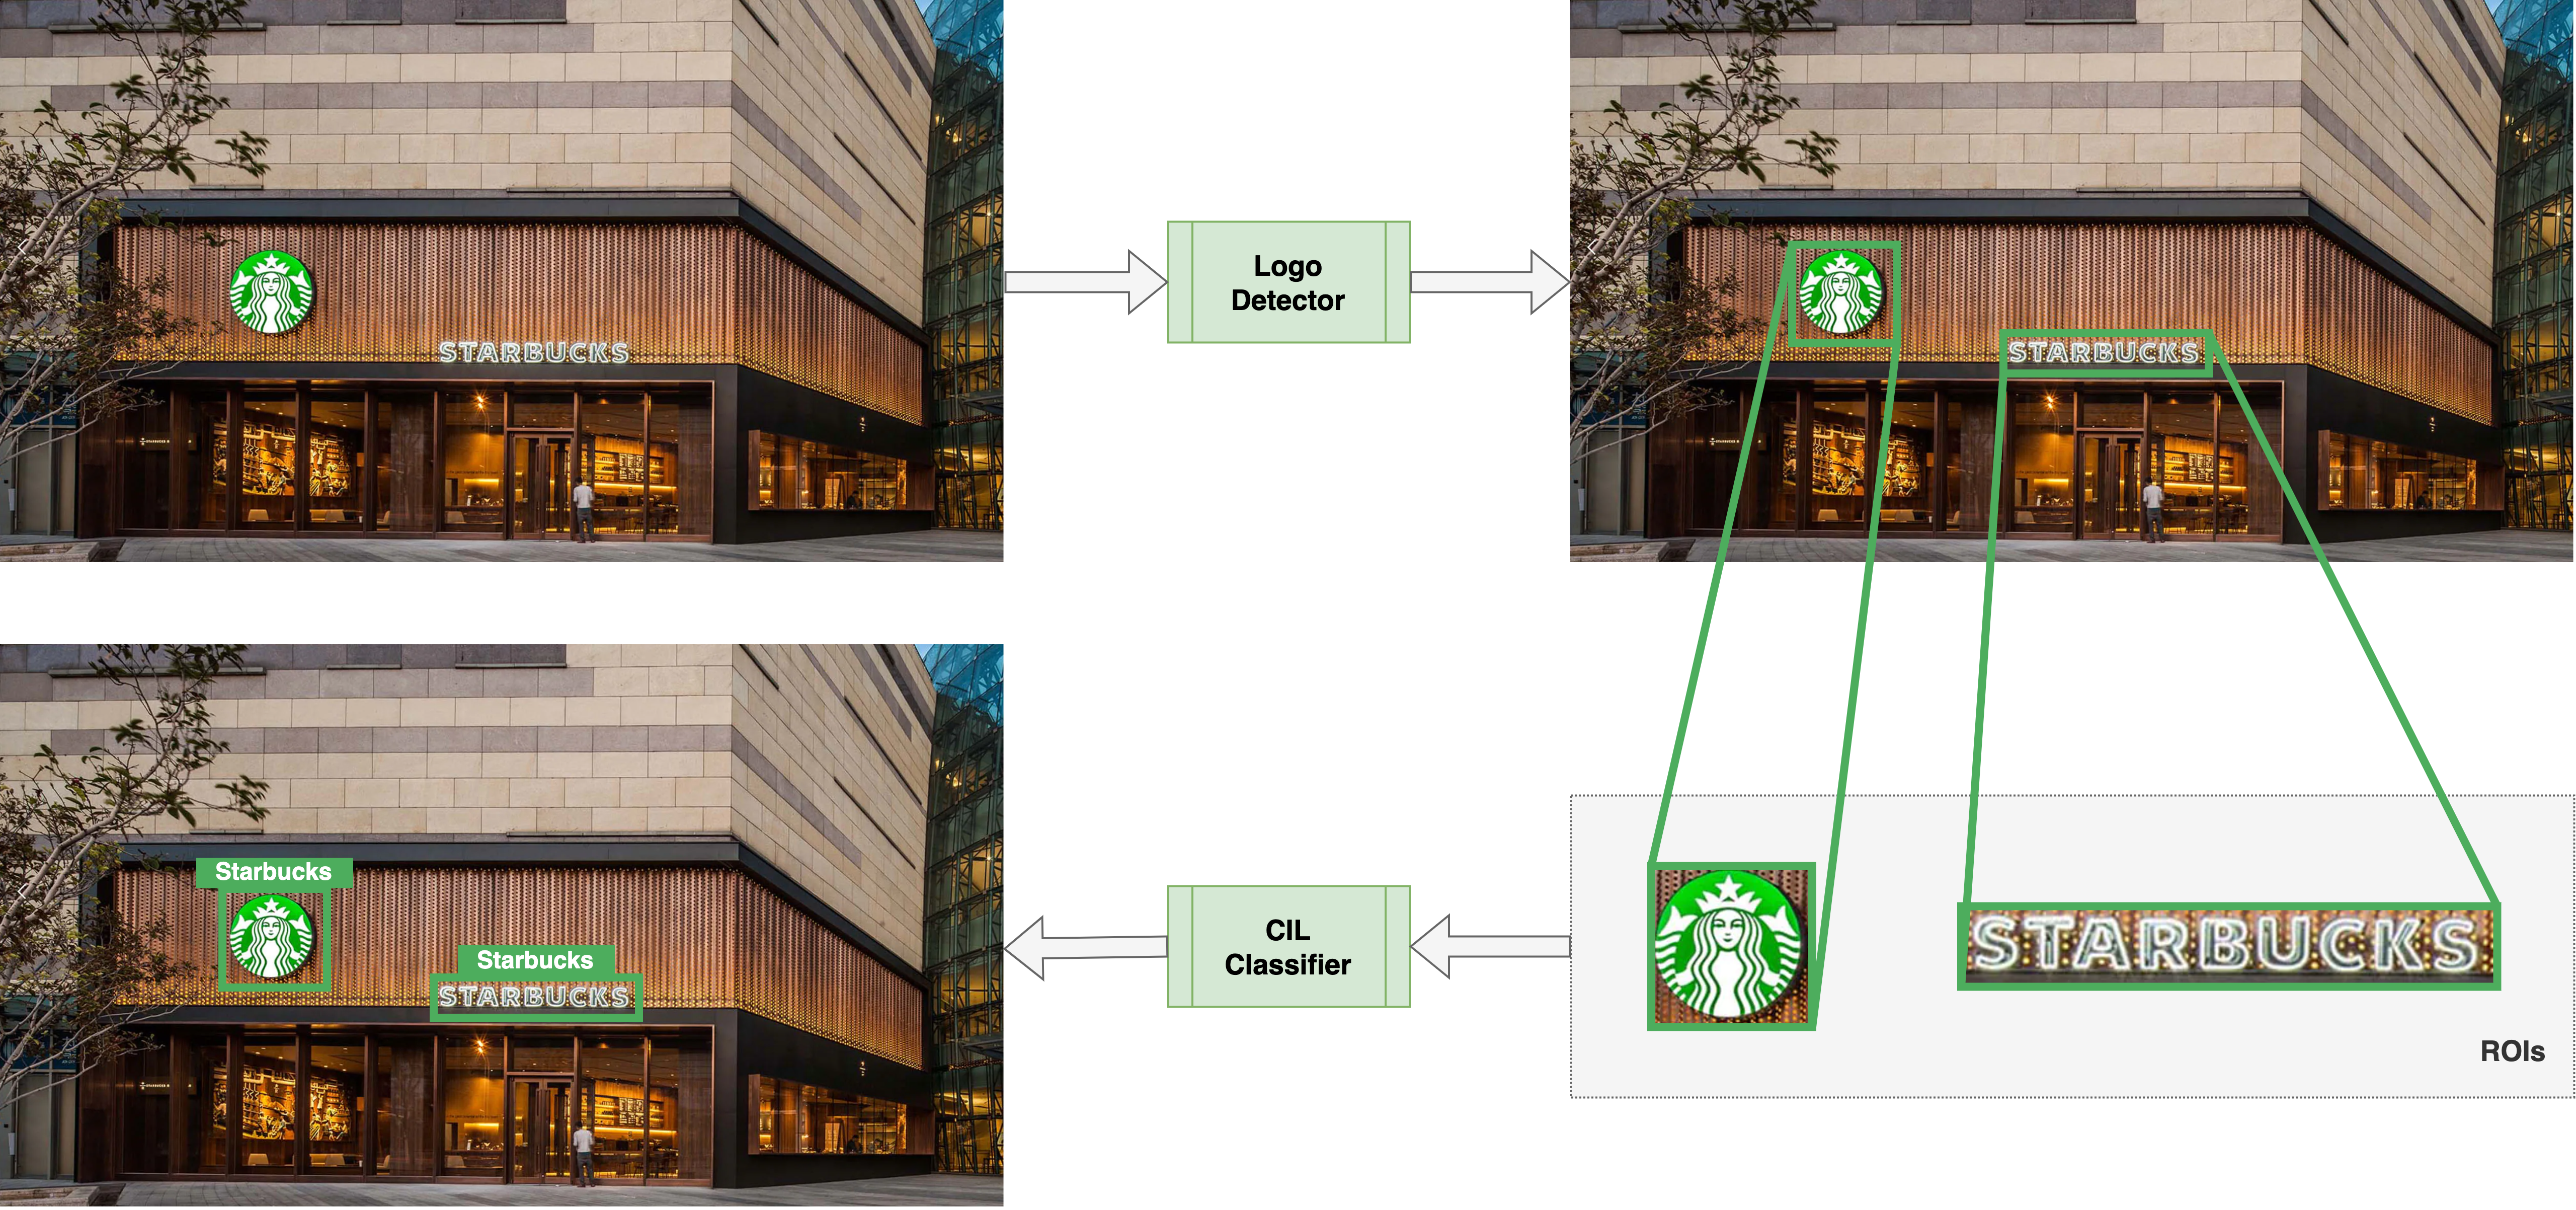
\includegraphics[width=\columnwidth]{images/roi+classification.drawio.png}
    \end{center}

	\caption{Pipeline of the system: the class-agnostic logo detector generates ROIs, then the classification is performed by the CIL classifier.}%
	\label{fig:roi_and_classification}%
\end{figure}

The detector used in the first step is a class-agnostic logo detector: it is a logo detector since we are not interested in the detection of objects other than logo; and it is class-agnostic since the number of detected classes is only one. In fact, in this first step the detector will be responsible for finding any generic logo (i.e., a single class) in the image. This is a crucial step if we seek to achieve incremental learning logo recognition, because in this way it is possible to decouple the detection from the recognition. If the logo detector localize any generic logo in the image, and delegates the actual recognition to the CIL classifier, there is no need to develop an incremental learning detector as well.


An important aspect of the classifier is the model size in terms of number of parameters. A big model comes with several disadvantages like longer time for the training phase, higher memory requirements and longer time to make inference. To this reason, a part of this work aims to decrease the number of parameters of the classifier using two different techniques. The first technique is described in \autoref{sec:method-pruning}, using masking and pruning described in \autoref{sec:masking-pruning} it aims to prune the model after the training of each incremental step, thus reducing the number of parameters. The second approach is the Knowledge Distillation (KD) described in \autoref{sec:method-kd}, where a smaller model is trained from scratch with the supervision of a bigger model trained on the same task.


\vspace{1.5\baselineskip}
This chapter describes all the details about the logo detector in \autoref{sec:method-roi} and continues with the classifier in \autoref{sec:method-classifier}. Then, in \autoref{sec:method-pruning} and \autoref{sec:method-kd} are discussed some techniques with the purpose to reducing the number of parameters of the model. In order to evaluate the drop in the terms of performance of the CIL classifier when compared to a standard close-set classification task (i.e. all the classes are available ath the beginning and there is no need to introduce new classes during time),
the chapter ends in \autoref{sec:method-baseline} with the introduction of different baselines.

The code develop during this thesis is available in the GitHub repository \footnote{GitHub repository relative to the code of developed in this thesis: \\ \href{https://github.com/gianlucagiudice/logo-detection-recognition}{https://github.com/gianlucagiudice/logo-detection-recognition}} linked below.


\section{Region proposal}
A key component of the system is the logo detector. Formally, this first step is an object detection task, where the objects we seek to detect are the logos in the image. The logo detector produces in output the coordinates of the bounding boxes corresponding to the logos in the image. The bounding boxes can be used to crop the portions of the images generating the regions of interest (ROIs). The ROIs corresponds to what the detector considers as any generic logo, and these can be directly used as input for the CIL model which classifies (i.e. recognize) the logo.


\label{sec:method-roi}
\subsection{YOLO}
The class-agnostic logo detector is based on YOLOv5m6 \cite{glenn_jocher_2021_5563715}.

Immagine delle diverse size di YOLO

Tabella delle diverse size di YOLO

\section{Classification}
\label{sec:method-classifier}
Given the ROIs, the classification of each cropped region is performed by a model trained using CIL techniques. To achieve this goal, the classifier is trained using the DER algorithm \cite{yan2021dynamically} described in \autoref{sec:der-algorithm}.

\subsection{ResNet-34}
The DER algorithm introduces a new feature extractor $\mathcal{F}_t$ at each incremental step. This feature extractor consists of a Convolutional Neural Network (CNN). In the developed system, the backbone of the CNN used as feature extractor is ResNet-34 \cite{he2016deep} pre-trained on ImageNet1000 \cite{deng2009imagenet}.

The peculiar aspect of the ResNet architecture are the Residual Connections, shown in \autoref{fig:residual-connection}.. These connections are a type of skip-connection that, instead of learning unreferenced functions, learn residual functions with respect to the layer inputs. Formally, denoting the desired underlying mapping as $\mathcal{H}(x)$, we let the stacked nonlinear layers fit another mapping of $\mathcal{F}(x) := \mathcal{H}(x) - x$. The original mapping is recast into $\mathcal{F}(x) + x$. 

The intuition is that it is easier to optimize the residual mapping than to optimize the original, unreferenced mapping. To the extreme, if an identity mapping were optimal, it would be easier to push the residual to zero than to fit an identity mapping by a stack of nonlinear layers \cite{he2016deep}.

The architecture of ResNet-34, shown in \autoref{table:resnet}, consists in multiple stacked building blocks. Each building block, represented by the brackets in \autoref{table:resnet}, adopt the residual connection described above.

\begin{table}
    \centering
    \begingroup
    
    \begin{tabular}{>{\centering\arraybackslash}p{.3\textwidth}|>{\centering\arraybackslash}p{.3\textwidth}|>{\centering\arraybackslash}p{.3\textwidth}}


        \hline
        \multicolumn{3}{c}{\textbf{ResNet-34 architecture}}\\
        \hline
        \textbf{Layer name} & \textbf{Output size} & \textbf{Layer} \\
        \hline
        \hline
        conv1 & $112 \times 122$ & $7 \times 7, 64,$ stride $2$ \\
        \hline
          & $56 \times 56$ & $3 \times 3$ max pool, stride $2$ \\
        \hline

        \[ \textrm{conv2\char`_x} \] &  \[56 \times 56 \] & \[\left[ \begin{array}{c} 3 \times 3, \, 64\\ 3 \times 3, \, 64  \end{array}\right] \times 3 \]\\
        \hline

        \[ \textrm{conv3\char`_x} \] &  \[28 \times 28 \] & \[\left[ \begin{array}{c} 3 \times 3, \, 128\\ 3 \times 3, \, 128  \end{array}\right] \times 4 \]\\
        \hline

        \[ \textrm{conv4\char`_x} \] &  \[14 \times 14 \] & \[\left[ \begin{array}{c} 3 \times 3, \, 256\\ 3 \times 3, \, 256  \end{array}\right] \times 6 \]\\
        \hline

        \[ \textrm{conv5\char`_x} \] &  \[7 \times 7 \] & \[\left[ \begin{array}{c} 3 \times 3, \, 512\\ 3 \times 3, \, 512  \end{array}\right] \times 3 \]\\
        \hline
        & $1000 \times 1$ & average pool \\
        \hline
        FC & $1000 \times 1$ & $1000$-d FC layer, softmax \\
        \hline
        \end{tabular}
    \endgroup
    \caption{Architecture of ResNet-34, the brackets represent}
    \label{table:resnet}
\end{table}



\begin{figure}%
	\centering
	\subfloat[\centering Residual learning: a building block]{{\includegraphics[width=0.45\textwidth]{images/residual-theory.png} }}%
	\hfill
	\subfloat[ An example of residual connection in a building block on a $56 \times 56$ feature maps. This building block corresponds to \textrm{conv2\char`_x} in \autoref{table:resnet} ]{{\includegraphics[width=0.45\textwidth]{images/residual-practice.png} }}%
	\caption{Residual connection in ResNet architecture \cite{he2016deep}.}%
	\label{fig:residual-connection}%
\end{figure}

\subsection{CIL classifier}
The classifier is developed in a CIL setup. In this way it is possible to recognize new logos by enriching the old knowledge. The algorithm used for CIL is the DER algorithm described in \autoref{sec:der-algorithm}. An implementation of the DER algorithm is given by PyCIL\footnote{PyCIL GitHub repository: \href{https://github.com/G-U-N/PyCIL}{https://github.com/G-U-N/PyCIL}}, and has been used as the starting for the development of the CIL classifier. All the changes performed to the implementation of DER in PyCIL are described in the following sections, and can be found in this\footnote{GitHub repository relative to the CIL model of this thesis: \\ \href{https://github.com/gianlucagiudice/PyCIL}{https://github.com/gianlucagiudice/PyCIL}} GitHub repository.


The implementation of DER in PyCIL reflects the description of the DER paper, the only change is relative to the third stage of the DER algorithm referred to as "Classifier Learning Stage" in \autoref{sec:der-algorithm}. In fact, in PyCIL the Classifier Learning Stage is performed using the WA described in \autoref{sec:wa-biased}; in this way it is possible to solve the problem of biased weights in the FC layer without the need to train the model further. It is important to point out that although this step of the original algorithm has been changed, the final performance reported by PyCIL is very similar to that obtained from the original DER paper (see \autoref{table:cil-results}).

\subsection{Regularization techniques}
In order to prevent overfitting
\subsection{Data Augmentation}
In order to prevent overfitting
\subsection{Optimizer}
In order to prevent overfitting


\subsection{Pruning}
in order to reduce the number of parameter has been implemented the amsking and pruning described in section.
\label{sec:method-pruning}
\section{Knowledge distillation}

\label{sec:method-kd}
\section{Proposed baseline for the classifier}
\label{sec:method-baseline}
\subsection{Baseline without incremental steps}
\subsection{ResNet-152 architecture}
\subsection{DER-based architecture}
\chapter{Experiments}
\label{chap:experiments}
This chapter presents the experiments designed to evaluate the system described in chapter \autoref{chap:methods}.
The chapter is structured as follows: \autoref{sec:exp-setup} specifies the setup used for the class incremental learning task; \autoref{sec:exp-cil} discusses the experiments related to the CIL model and \autoref{sec:exp-det} those related to the logo detector; \autoref{sec:exp-kd} describes the experiments relative to the KD; finally, \autoref{sec:exp-end2end} presents the results of experiments combining the logo detector with the CIL classifier.

\section{Setup}
\label{sec:exp-setup}
The developed system is tested considering two different CIL setups: in the first setup, the system is tested on a subset of 100 classes out of the total 2993 in the dataset; in the second setup, the model's scaling capabilities are tested considering the entire dataset. Specifically, the CIL configuration is the following:
\begin{enumerate}
    \item \textbf{100 Classes}: 100 classes are extracted from the initial dataset. For the experiments, a distinction is made between the case in which these classes are extracted randomly or are taken the 100 classes with the highest number of images.
    
    Out of these 100 classes, 30 are used for the initial task, then the remaining 70 classes are added 10 at a time through 7 incremental learning iterations.

    \item \textbf{2993 Classes (entire dataset)}: for experiments which consider the entire dataset, the first 1000 classes are used for the initial task, then follows 8 iterations of incremental learning, each adding 250 new classes.
\end{enumerate}

The train, validation and test set are built from the individual classes. For each of these, the instances are divided as follows:
\begin{itemize}
    \item \textbf{Train set}: 70 \%
    \item \textbf{Validation set}: 10 \%
    \item \textbf{Test set}: 20 \%
\end{itemize}


\section{Classifier: CIL model}
\label{sec:exp-cil}
Top-k accuracy is used to evaluate the performance of the CIL model, focusing on cases with $k=1$ and $k=5$.
Using this performance metric, a classification is considered correct if the label is present among the first $k$ predictions to which the model assigns the highest probability. Thus, the accuracy is calculated as the percentage of the correct predictions.

\subsection{100 Classes}
\subsubsection{100 Classes randomly sampled}
For the first experiments, the 100 classes are randomly sampled from the 2993 classes in the dataset, then the classifier is evaluated on the test set according to the CIL setup described in \autoref{sec:exp-setup}. 

As detailed in \autoref{sec:der-algorithm}, the DER algorithm saves some examples of the 'old' classes and reuses these examples during incremental learning iterations. In the following experiments, the memory dedicated to each old class is of 100 samples.

The first group of experiments aims to compare two types of architecture: ResNet-34 and ResNet-50. In addition, the cases where CNNs are pre-trained on ImageNet or not are also considered. For these experiments, the optimizer is SGD and neither regularization of the model via the dropout layer nor data augmentation is used.

The results of the experiments in picture \autoref{fig:exp1} and table \autoref{table:exp1}, reporting the top-1 and top-5 accuracy of the models at varying CIL tasks on the test set, show that pre-trained CNNs perform better, but there is not much difference between ResNet-34 and ResNet-50. For this reason, the architecture chosen for the experiments to follow is ResNet-34, so as to have a slightly smaller network than ResNet-50, and the network is pre-trained on ImageNet.

\begin{figure}[H]
    \centering
	\subfloat[\centering Top-1 accuracy]{{\includegraphics[width=0.80\textwidth]{images/exp/exp1-top1.png} }}%
    \qquad
    \subfloat[\centering Top-5 accuracy]{{\includegraphics[width=0.80\textwidth]{images/exp/exp1-top5.png} }}%
    \caption{Top-1 and Top-5 accuracy of the models at varying CIL tasks on the test set.}%
	\label{fig:exp1}%
\end{figure}

\begin{table}[H]
    \centering
    \centerline{
    \begin{tabular}{c|c|c|c|c}
        \hline
        \textbf{Model} &
        \textbf{Backbone} &
        \textbf{Pre-trained} &
        \textbf{Top-1} & 
        \textbf{Top-5} \\
        \textbf{name} &
        &
        &
        \textbf{acc. (\%)} & 
        \textbf{acc. (\%)} \\
        \hline
        \hline
resnet34-SGD-nopretrained-drop0 &ResNet-34&no& 52.97 & 87.02\\
resnet34-SGD-pretrained-drop0 &ResNet-34&yes& \textbf{60.37} & \textbf{93.19}\\
resnet50-SGD-nopretrained-drop0 &ResNet-50&no& 50.43 & 86.28\\
resnet50-SGD-pretrained-drop0 &ResNet-50&yes& 58.54 & 92.59\\
        \hline        
    \end{tabular}}
    \caption{Top-1 and Top-5 accuracy of the models at task 7.}
    \label{table:exp1}
\end{table}


Other useful insights can be derived from the training history of a task (e.g. Task 7) which reports the top-1 accuracy on the training and validation set. In fact, as we can see from \autoref{fig:exp1-train_val} the accuracy on the training set is much higher than the validation set, which is a clear sign of overfitting of the model.

\begin{figure}[H]
    \centering
    \subfloat[\centering Accuracy on the training set]{{\includegraphics[width=0.80\textwidth]{images/exp/exp1-train.png} }}%
    \qquad
    \centering
    \subfloat[\centering Accuracy on the validation set]{{\includegraphics[width=0.80\textwidth]{images/exp/exp1-val.png} }}%
    \caption{Comparison of the accuracy at each training epoch at task 7 between the training and validation set.}%

        \label{fig:exp1-train_val}%
\end{figure}

\newpage
\subsubsection{Regularization and data augmentation}
Following the analysis discussed above, it is necessary to regularize the model.
To do so, the next experiments are performed using the dropout layer (see \autoref{sec:methods-dropout}) and data augmentation (see \autoref{sec:methods-augment}). As said before, the backbone of each model is ResNet-34 and each one is pre-trained on ImageNet.

As expected, the performance at each task is higher than before, as shown in \autoref{fig:exp2}. Analyzing \autoref{fig:exp2-train_val}, the accuracy on the train and validation set at task 7 (the same as before), the training accuracy is lower than models without regularization, but the validation accuracy is higher. This is a sign that the regularization works as intended.

As shown in \autoref{table:exp2}, the top-1 accuracy of the best regularized model which adopting data augmentation is 7\% higher than that without regularization and data augmentation.


\begin{table}[H]
    \centering
    \centerline{
    \begin{tabular}{c|c|c|c|c}
        \hline
        \textbf{Model} &
        \textbf{Data} &
        \textbf{Dropout} &
        \textbf{Top-1} & 
        \textbf{Top-5} \\
        \textbf{name} &
        \textbf{augm.} &
        \textbf{rate} &
        \textbf{acc. (\%)} & 
        \textbf{acc. (\%)} \\
        \hline
        \hline
SGD-nopretrained-drop0 &no&0.0& 52.97 & 87.02\\
SGD-pretrained-drop0 &no&0.0& 60.37 & 93.19\\
\hline
SGD-pretrained-drop0.1-augmented&yes&0.1&	67.17&\textbf{98.15}\\
SGD-pretrained-drop0.3-augmented&yes&0.3&\textbf{67.28}&	97.3\\
SGD-pretrained-drop0.5-augmented&yes&0.5&65.57&	96.24\\
        \hline        
    \end{tabular}}
    \caption{Regularized models with data augmentation. Top-1 accuracy at task 7.}
    \label{table:exp2}
\end{table}

\newpage
\begin{figure}[H]
	\centering
	\subfloat[\centering Top-1 accuracy]{{\includegraphics[width=0.80\textwidth]{images/exp/exp2-top1.png} }}%
    \qquad
	\subfloat[\centering Top-5 accuracy]{{\includegraphics[width=0.80\textwidth]{images/exp/exp2-top5.png} }}%
	\caption{Top-1 and Top-5 accuracy of the regularized models using data augmentation.}%
	\label{fig:exp2}%
\end{figure}

\begin{figure}[H]
	\centering
	\subfloat[\centering Accuracy on the training set]{{\includegraphics[width=0.80\textwidth]{images/exp/exp2-train.png} }}%
    \qquad
	\subfloat[\centering Accuracy on the validation set]{{\includegraphics[width=0.80\textwidth]{images/exp/exp2-val.png} }}%
	\caption{Regularized models with data augmentation: comparison of the top-1 accuracy at each training epoch at task 7 between training and validation.}%
	\label{fig:exp2-train_val}%
\end{figure}

\newpage
\subsubsection{Type 1 baseline}
To compare the performance of the CIL model with a standard non-incremental learning setup, a baseline is trained using the same train/validation/test split of the CIL model. In particular, this experiment exploits the definition of 'type 1 baseline' described in \autoref{sec:method-baseline1}, i.e. it uses the DER algorithm and trains the model at task 0 with all 100 classes. Analogous to the CIL model, the baseline uses data augmentation, the SGD optimizer, a dropout layer before the FC layer and ResNet-34 pre-trained on ImageNet as backbone for the feature extract.

The performance comparison between the CIL models and the baselines is compared considering the top-1 accuracy on the test set. The results are shown in \autoref{table:baseline1}. As we can see, the best CIL model performs better than the best baseline, which is the opposite of what one might expect. However, as we can see from \autoref{table:baseline1-params}, this is due to the difference in the number of parameters described in \autoref{sec:method-baseline1}. For this reason, in the section section the CIL models are compared using a different type of baseline.

\begin{table}[H]
    \centering
    \centerline{
    \begin{tabular}{c|c|c|c}
        \hline
        \textbf{Model} &
        \textbf{Dropout} &
        \textbf{Top-1} & 
        \textbf{Top-5} \\
        \textbf{name} &
        \textbf{rate} &
        \textbf{acc. (\%)} & 
        \textbf{acc. (\%)} \\
        \hline
\hline
SGD-pretrained-drop0.1-augmented&0.1&67.17\\
SGD-pretrained-drop0.3-augmented&0.3&\textbf{67.28}\\
SGD-pretrained-drop0.5-augmented&0.5&65.57\\
\hline
BASELINE\_1-pretrained-drop0.1-augmented&0.1&63.04\\
BASELINE\_1-pretrained-drop0.3-augmented&0.3&61.15\\
BASELINE\_1-pretrained-drop0.5-augmented&0.5&57.14\\
\hline 
    \end{tabular}}
    \caption{Performance comparison between the CIL model and the type 1 baseline. Top-1 accuracy at task 7 (CIL model) and task 0 (baseline).}
    \label{table:baseline1}
\end{table}

\begin{table}[H]
    \centering
    \centerline{
    \begin{tabular}{c|c}
        \hline
        \textbf{Model} &
        \textbf{\#Params} \\
        \textbf{name} &
        \textbf{(M)} \\
        \hline
\hline
SGD-pretrained-drop0.1-augmented&170\\
SGD-pretrained-drop0.3-augmented&170\\
SGD-pretrained-drop0.5-augmented&170\\
\hline
BASELINE\_1-pretrained-drop0.1-augmented&21\\
BASELINE\_1-pretrained-drop0.3-augmented&21\\
BASELINE\_1-pretrained-drop0.5-augmented&21\\
\hline 
    \end{tabular}}
    \caption{Number of model parameters between the CIL model and the typ 1 baseline. Number of parameters at task 7 (CIL model) and task 0 (baseline).}
    \label{table:baseline1-params}
\end{table}

\subsubsection{Top-100 Classes}
\label{sec:cil-top100}
In order to assess the extent to which those classes with few examples contribute to performance deterioration, the next experiments are carried out by considering only the top-100 classes, i.e. those with the largest number of examples (see the left-hand side of the distribution in \autoref{fig:logodet-dist}). This is useful to be aware of how much the model is limited in performance by the dataset.

Considering the regularized models and data augmentation, models trained on 100 randomly sampled classes and those trained on the top-100 classes are compared in \autoref{fig:exp3} and \autoref{table:exp3}. As we can see, even if the top-5 accuracy does not change between the two cases, considering the top-1 accuracy there is a drastic improvement in performance. This is a clear sign that classes with few examples deteriorate performance a lot.

\begin{table}[H]
    \centering
    \centerline{
    \begin{tabular}{c|c|c|c|c}
        \hline
        \textbf{Model} &
        \textbf{Dropout} &
        \textbf{Sampling} &
        \textbf{Top-1} & 
        \textbf{Top-5} \\
        \textbf{name} &
        \textbf{rate} &
        \textbf{method} &
        \textbf{acc. (\%)} & 
        \textbf{acc. (\%)} \\
        \hline
        \hline
drop0.1-augmented&0.1&random&	67.17&98.15\\
drop0.3-augmented&0.3&random&67.28&	97.3\\
drop0.5-augmented&0.5&random&65.57&	96.24\\
\hline
drop0.1-augmented-onlytop&0.1&top-100&\textbf{89.1}&\textbf{96.59}\\
drop0.3-augmented-onlytop&0.3&top-100&88.14&96.39\\
drop0.5-augmented-onlytop&0.5&top-100&87.6&95.92\\
        \hline
    \end{tabular}}
    \caption{Comparison of models trained on 100 randomly sampled classed and top-100 classes. Top-1 accuracy at task 7.}
    \label{table:exp3}
\end{table}
\newpage
\begin{figure}[H]
	\centering
	\subfloat[\centering Top-1 accuracy]{{\includegraphics[width=0.80\textwidth]{images/exp/exp3-top1.png} }}%
    \qquad
	\subfloat[\centering Top-5 accuracy]{{\includegraphics[width=0.80\textwidth]{images/exp/exp3-top5.png} }}%
	\caption{Comparison of models trained on 100 randomly sampled classed and top-100 classes.}%
	\label{fig:exp3}%
\end{figure}

\newpage
\subsubsection{Introduction of Adam optimizer}
The next experiments aim to compare the SGD (see \autoref{sec:sgd_opt}) and Adam (see \autoref{sec:adam_opt}) optimizers. Considering the regularized models, data augmentation and the top-100 classes, the result of this comparison is shown in \autoref{fig:exp4} and \autoref{table:exp4}.


As we can see from the results shown in \autoref{table:exp4}, the top-1 accuracy at task 7 improves by more than 6\% using the Adam as the optimization algorithm. 
In addition to the performance aspect, the training history in \autoref{fig:exp4-train_val} shows that Adam leads to faster convergence. In fact the models trained with this algorithm achieve the highest value of top-1 accuracy on the validation set after only a few training epochs.

\begin{table}[H]
    \centering
    \centerline{
    \begin{tabular}{c|c|c|c|c}
        \hline
        \textbf{Model} &
        \textbf{Dropout} &
        \textbf{Optimizer} &
        \textbf{Top-1} & 
        \textbf{Top-5} \\
        \textbf{name} &
        \textbf{rate} &
        \textbf{method} &
        \textbf{acc. (\%)} & 
        \textbf{acc. (\%)} \\
        \hline
        \hline
SGD-drop0.1-augmented-onlytop&0.1&SGD&89.1&96.59\\
SGD-drop0.3-augmented-onlytop&0.3&SGD&88.14&96.39\\
SGD-drop0.5-augmented-onlytop&0.5&SGD&87.6&95.92\\
\hline
adam-drop0.1-augmented-onlytop&0.1&Adam&92.15&97.92\\
adam-drop0.3-augmented-onlytop&0.3&Adam&91.55&97.75\\
adam-drop0.5-augmented-onlytop&0.5&Adam&\textbf{95.04}&\textbf{98.4}\\
        \hline
    \end{tabular}}
    \caption{Comparison of models trained using SGD and Adam. Top-1 accuracy at task 7.}
    \label{table:exp4}
\end{table}

\newpage

\begin{figure}[H]
	\centering
	\subfloat[\centering Top-1 accuracy]{{\includegraphics[width=0.80\textwidth]{images/exp/exp4-top1.png} }}%
    \qquad
	\subfloat[\centering Top-5 accuracy]{{\includegraphics[width=0.80\textwidth]{images/exp/exp4-top5.png} }}%
	\caption{Comparison of models trained using SGD and Adam.}%
	\label{fig:exp4}%
\end{figure}

\begin{figure}[H]
	\centering
	\subfloat[\centering Accuracy on the training set]{{\includegraphics[width=0.80\textwidth]{images/exp/exp4-train.png} }}%
    \qquad
	\subfloat[\centering Accuracy on the validation set]{{\includegraphics[width=0.80\textwidth]{images/exp/exp4-val.png} }}%
	\caption{Models trained using SGD and Adam: comparison of the accuracy at each training epoch at task 7 between the validation and training set.}%
	\label{fig:exp4-train_val}%
\end{figure}

\newpage


\newpage
\subsubsection{Type 2 baseline}
To address the problems relative to the type 1 baseline, the models tested in the previous section are compared to the 'type 2 baseline' described in \autoref{sec:method-baseline2}. This new baseline is trained on the same dataset used for CIL models and consists in fine-tuning ResNet-152 pretrained on ImageNet to the task of logo classification. This new baseline uses data augmentation, a dropout layer before the FC layer and the Adam optimizer.

Considering the top-1 and top-5 accuracy on the test set, the performance of CIL models and the type 2 baselines is compared in \autoref{table:baseline2}.
As we can see, the performance of the best CIL model is very similar to that of the baseline, but the latter still performs worse, even if slightly.
Although this new baseline mitigates the problem of the number of model parameters, this is still present, as shown in \autoref{table:baseline2-params}.

\begin{table}[H]
    \centering
    \centerline{
    \begin{tabular}{c|c|c}
        \hline
        \textbf{Model} &
        \textbf{Dropout} &
        \textbf{Top-1} \\
        \textbf{name} &
        \textbf{rate} &
        \textbf{acc. (\%)} \\
        \hline
\hline
adam-drop0.1-augmented-onlytop&0.1&92.15\\
adam-drop0.3-augmented-onlytop&0.3&91.55\\
adam-drop0.5-augmented-onlytop&0.5&\textbf{95.04}\\
\hline
BASELINE\_2-drop0.1-augmented-onlytop&0.1&82.35\\
BASELINE\_2-drop0.3-augmented-onlytop&0.3&94.11\\
BASELINE\_2-drop0.5-augmented-onlytop&0.5&88.23\\
\hline 
    \end{tabular}}
    \caption{Performance comparison between the CIL model and the type 2 baseline. Top-1 accuracy tested on 100 classes.}
    \label{table:baseline2}
\end{table}

\begin{table}[H]
    \centering
    \centerline{
    \begin{tabular}{c|c}
        \hline
        \textbf{Model} &
        \textbf{\#Params} \\
        \textbf{name} &
        \textbf{(M)} \\
        \hline
adam-drop0.1-augmented-onlytop&170\\
adam-drop0.3-augmented-onlytop&170\\
adam-drop0.5-augmented-onlytop&170\\
\hline
BASELINE\_2-drop0.1-augmented-onlytop&60\\
BASELINE\_2-drop0.3-augmented-onlytop&60\\
BASELINE\_2-drop0.5-augmented-onlytop&60\\
\hline 
    \end{tabular}}
    \caption{Number of model parameters between the CIL model and the typ 2 baseline.}
    \label{table:baseline2-params}
\end{table}

\newpage
\subsubsection{Type 3 baseline}
This third baseline, 'type 3 baseline' aims to solve the problem of the number of model parameters. In fact, this approach, described in \autoref{sec:method-baseline3}, defines the baseline architecture using the DER algorithm in the exact same setup as the CIL classifier, thus having an identical architecture of the CIL model and the baseline.
This ensures that the number of model parameters is the same.
Therefore, the baseline is trained using the same dataset, data augmentation, regularization, and the Adam optimizer.

The performance between the CIL models and this new baseline is compared considering the top-1 on the test set. As we can see from \autoref{table:baseline3}, the type 3 baseline achieves better performance than the CIL model.

This makes it possible to compare the actual drop in performance using an incremental learning setup compared to a standard setup.
As shown in \autoref{table:baseline3}, this gap is present, with a 3\% drop in top-1 accuracy, but it is expected using an incremental learning setup.
However, a 3\% drop is acceptable when considering the advantages of an incremental learning approach.

\begin{table}[H]
    \centering
    \centerline{
    \begin{tabular}{c|c|c|c}
        \hline
        \textbf{Model} &
        \textbf{Dropout} &
        \textbf{Top-1} \\
        \textbf{name} &
        \textbf{rate} &
        \textbf{acc. (\%)} \\
        \hline
\hline
adam-drop0.1-augmented-onlytop&0.1&92.15\\
adam-drop0.3-augmented-onlytop&0.3&91.55\\
adam-drop0.5-augmented-onlytop&0.5&95.04\\
\hline\
BASELINE\_3-drop0.1-augmented-onlytop&0.1&\textbf{98.52}\\
BASELINE\_3-drop0.3-augmented-onlytop&0.3&97.05\\
BASELINE\_3-drop0.5-augmented-onlytop&0.5&97.64\\
\hline 
    \end{tabular}}
    \caption{Top-1 accuracy of the CIL model and the type 3 baseline consider all the 100 classes of the test set.}
    \label{table:baseline3}
\end{table}

\newpage
\subsubsection{Pruning (100 classes)}
An important aspect discussed in \autoref{sec:method-pruning} is the number of model parameters. All the models tested up to this point add approximately 22 million parameters with each new incremental iteration of learning, thus reaching 170 million parameters at task 7 (22 million for the initial task and 7 iterations of incremental learning).

The following experiments are designed to assess the pruning capacity of the channel-level masks and the drop in performance obtained by using this method. To this end, the pruned models are compared to those described in the previous section. An important difference in the training procedure of the pruned model is to monitor the loss on the validation set instead of the validation accuracy. Since the validation loss decreases with increasing sparsity of the model, we want to encourage a sparser model given the same accuracy on the validation set.

The results regarding the performance comparison are shown in \autoref{fig:exp5} and \autoref{table:exp5}. As we can see, the drop in performance is negligible, with some pruned models performing even better than un-pruned ones. This can be explained by considering pruning as a regularization technique, in fact, the number of parameters reduced (effectively reducing the Vapnik-Chervonenkis dimension \cite{vapnik1999nature}). However, it is important to emphasize that these models are trained considering the top-100 classes, so it is essential to test the scalability of the models, and also of pruning, to the entire dataset.


\begin{figure}[H]
	\centering
	\subfloat[\centering Top-1 accuracy]{{\includegraphics[width=0.80\textwidth]{images/exp/exp5-top1.png} }}%
    \qquad
	\subfloat[\centering Top-5 accuracy]{{\includegraphics[width=0.80\textwidth]{images/exp/exp5-top5.png} }}%
	\caption{Performance comparison between the pruned model and standard model.}%
	\label{fig:exp5}%
\end{figure}

\begin{table}[H]
    \centering
    \centerline{
    \begin{tabular}{c|c|c|c|c}
        \hline
        \textbf{Model} &
        \textbf{Dropout} &
        \textbf{Pruning} &
        \textbf{Top-1} & 
        \textbf{Top-5} \\
        \textbf{name} &
        \textbf{rate} &
        &
        \textbf{acc. (\%)} & 
        \textbf{acc. (\%)} \\
        \hline
        \hline
drop0.1-augmented-onlytop&0.1&no&92.15&97.92\\
drop0.3-augmented-onlytop&0.3&no&91.55&97.75\\
drop0.5-augmented-onlytop&0.5&no&\textbf{95.04}&\textbf{98.4}\\
\hline
PRUNED-drop0.1-augmented-onlytop&0.1&yes&92.58&96.96\\
PRUNED-drop0.3-augmented-onlytop&0.3&yes&92.05&96.29\\
PRUNED-drop0.5-augmented-onlytop&0.5&yes&91.45&95.67\\
        \hline
    \end{tabular}}
    \caption{Performance comparison between the pruned models and the un-pruned ones. Top-1 accuracy at task 7.}
    \label{table:exp5}
\end{table}

The result of pruning regarding the number of parameters is shown in \autoref{fig:exp5-params} and \autoref{table:exp5-params}. As we can see, this technique is very effective. The final number of model parameters is reduced by almost a factor of 5x, the models not using pruning already exceed the total number of parameters of those using pruning for task 1 (43 for the un-pruned vs. 32 for pruned approx.).

\begin{table}[ht]
    \begin{minipage}[b]{0.49\linewidth}
        \centering
        \includegraphics[width=1\linewidth]{images/exp/exp5-params.png}
        \captionof{figure}{Number of model parameters at each task using the pruning technique.}
        \label{fig:exp5-params}
    \end{minipage}
    \hfill
    \begin{minipage}[b]{0.49\linewidth}
        \centering
        \begin{tabular}{c|c}
            \hline
            \textbf{Model} &
            \textbf{\#Params} \\
            \textbf{name} &
            \textbf{(M)} \\
            \hline
            \hline
UNPRUNED-drop0.1&170\\
UNPRUNED-drop0.3&170\\
UNPRUNED-drop0.5&170\\
\hline
PRUNED-drop0.1&34.08\\
PRUNED-drop0.3&32.48\\
PRUNED-drop0.5&36.41\\
            \hline
        \end{tabular}
            \caption{Number of model parameters at task 7.}
            \label{table:exp5-params}
    \end{minipage}
\end{table}

Other interesting insights emerge by analyzing the training history of the models at task 0. The loss function of the DER algorithm (\autoref{eq:final_der_loss}) is defined as the sum of: the loss of the classifier, the loss of the auxiliary classifier and loss related to the pruning masks. In \autoref{fig:exp5-loss} we can see the classification loss (c), the sparsity loss (d) and the final loss (b) of the model for each training epoch at task 0. Initially, the loss (c) tends to decrease, but as the training epochs advance, the sparsity loss (d) increasingly limits the channels of the convolutional layers. This leads to a continuous decrease in parameters, but the classification (c) is affected considerably. The deterioration in performance can also be seen in the top-1 accuracy (a) on the validation set.


\begin{figure}[H]
	\centering
	\subfloat[\centering Top-1 accuracy]{{\includegraphics[width=0.50\textwidth]{images/exp/exp5-val_acc.png} }}%
    
	\subfloat[\centering Final loss]{{\includegraphics[width=0.50\textwidth]{images/exp/exp5-val_loss.png} }}%
    
	\subfloat[\centering Classification loss]{{\includegraphics[width=0.50\textwidth]{images/exp/exp5-val_clf.png} }}%
    
	\subfloat[\centering Sparsity loss]{{\includegraphics[width=0.50\textwidth]{images/exp/exp5-val_spars.png} }}%
	\caption{Training history of the pruned model on the validation set at task 0.}%
	\label{fig:exp5-loss}%
\end{figure}


\subsection{2993 Classes}
\label{sec:whole_dataset_clf}

The following experiments test the scalability capabilities of the model. In fact, in this section, models will be trained on 2993 classes, i.e. the entire dataset.

\subsubsection{Varying the memory size}
Another important factor for testing the scalability of the model is the number of stored examples for old classes. Indeed, when many classes are introduced, it is necessary to limit the memory used to save old examples.
In this first section, the models are trained by varying the size of the memory used by the models to store examples of the old classes. The memory size is tested using: 50, 20 and 10 examples.

Regarding the other specifications of the model, it is trained according to the best results obtained previously with the experiments on 100 classes. Thus, the architecture of each feature extractor is ResNet-34 pretrained on ImageNet, the optimizer is Adam, regularization with a dropout layer is used as well as data augmentation, but initially no pruning is performed.

The results of the experiments are shown in \autoref{fig:exp6} and \autoref{table:exp6}.
As we can see, the models scale fairly well over the entire dataset, as a comparison of the setup of 100 classes shown in \autoref{table:exp5}, the drop in performance is only about 8\%, even though the examples stored in the setup of 2993 classes are 1/10 than before. As expected, the more samples stored for incremental learning iterations, the better the overall accuracy. The total number of examples stored by each model at task 8 is shown in \autoref{table:exp6-memsize}.

\begin{table}[H]
    \centering
    \centerline{
    \begin{tabular}{c|c|c|c|c}
        \hline
        \textbf{Model} &
        \textbf{Dropout} &
        \textbf{Mem.} &
        \textbf{Top-1} & 
        \textbf{Top-5} \\
        \textbf{name} &
        \textbf{rate} &
        \textbf{size} &
        \textbf{acc. (\%)} & 
        \textbf{acc. (\%)} \\
        \hline
        \hline
CIL\_2993-mem10-drop0.5-adam&0.1&10&87.2&92.19\\
CIL\_2993-mem20-drop0.5-adam&0.1&20&88.47&92.58\\
CIL\_2993-mem50-drop0.5-adam&0.1&50&\textbf{89.22}&\textbf{92.97}\\
        \hline
    \end{tabular}}
    \caption{Performance of the models at each incremental task trained on the entire dataset using different dimensions of memory size. Top-1 accuracy at task 8.}
    \label{table:exp6}
\end{table}


\begin{table}[H]
    \centering
    \begin{tabular}{c|c|c}
        \hline
        \textbf{Model} &
        \textbf{Mem.} &
        \textbf{\# Total saved} \\
        \textbf{name} &
        \textbf{per class} &
        \textbf{examples (K)} \\
        \hline
        \hline
CIL\_2993-mem10-drop0.5-adam&10&102\\
CIL\_2993-mem20-drop0.5-adam&20&53\\
CIL\_2993-mem50-drop0.5-adam&50&29\\
        \hline
    \end{tabular}
    \caption{Number of total examples stored by each model at task 8.}
    \label{table:exp6-memsize}
\end{table}


\begin{figure}[H]
	\centering
	\subfloat[\centering Top-1 accuracy]{{\includegraphics[width=0.80\textwidth]{images/exp/exp6-top1.png} }}%
    \qquad
	\subfloat[\centering Top-5 accuracy]{{\includegraphics[width=0.80\textwidth]{images/exp/exp6-top5.png} }}%
	\caption{Performance of the models at each incremental task trained on the entire dataset using different dimensions of memory size.}%
	\label{fig:exp6}%
\end{figure}

\newpage

\subsubsection{Type 3 baseline (2993 classes)}
As in the case of 100 classes, the performance of the CIL models is compared with the type 3 baseline (see \autoref{sec:method-baseline3}). For this purpose, the baseline is trained considering the same dataset used to train the models in the previous section.
Note that in the case of the baseline, there is no need to use a memory for the old classes since the incremental learning setup does not hold.
 
The comparison of top-1 accuracy between CIL models and baselines is shown in \autoref{table:baseline3-2993}.
Osservazioni\todo{Osservazioni}


\begin{table}[H]
    \centering
    \centerline{
    \begin{tabular}{c|c|c|c}
        \hline
        \textbf{Model} &
        \textbf{Dropout} &
        \textbf{Mem.} &
        \textbf{Top-1}\\
        \textbf{name} &
        \textbf{rate} &
        \textbf{size} &
        \textbf{acc. (\%)} \\
        \hline
\hline
CIL\_2993-mem10-drop0.5-adam&0.1&10&87.2\\
CIL\_2993-mem20-drop0.5-adam&0.1&20&88.47\\
CIL\_2993-mem50-drop0.5-adam&0.1&50&89.22\\
\hline\
BASELINE\_3-2993classes-drop0.1&0.1&-&-\\
BASELINE\_3-2993classes-drop0.3&0.3&-&-\\
BASELINE\_3-2993classes-drop0.5&0.5&-&-\\
\hline 
    \end{tabular}}
    \caption{Top-1 accuracy of the CIL model and the type 3 baseline consider all the 100 classes of the test set.}
    \label{table:baseline3-2993}
\end{table}

\newpage

\subsubsection{Pruning (2993 classes)}
\label{sec:pruning-entire}
Similarly to the setup with 100 classes, the pruning strategy is tested for models trained on the entire dataset. As we can see from \autoref{fig:exp7} and \autoref{table:exp7}, when using the pruning in combination to the Weight Aligning (WA), the performance drops dramatically. Therefore, only for models using pruning, WA is disabled.

In contrast to the experiments on 100 classes, now pruning results in poor performance, in fact the drop in accuracy is considerable compared to those models without pruning. Even considering the case using 50 samples for the pruning model, performance deteriorates by almost 20\%.

Regarding the number of parameters, even in the setup with 2993 classes the model is reduced in size considerably. As we can see from \autoref{table:exp7-params}, however, the pruning factor corresponds to approximately 3x compared to the 5x achieved in the previous setup.

In conclusion, the pruning strategy is not effective in the case of models trained on the entire dataset. For this reason, the KD is used and the result of the experiments is shown in \autoref{sec:exp-kd}.

\begin{table}[H]
    \centering
    \begin{tabular}{c|c|c|c|c|c}
        \hline
        \textbf{Model} &
        \textbf{Mem.} &
        \textbf{WA} &
        \textbf{Pruning} &
        \textbf{Top-1} & 
        \textbf{Top-5} \\
        \textbf{name} &
        \textbf{size} &
        &
        &
        \textbf{acc. (\%)} & 
        \textbf{acc. (\%)} \\
        \hline
        \hline
UNPRUNED-WA-mem10-drop0.5&10&yes&no&87.2&92.19\\
UNPRUNED-WA-mem20-drop0.5&20&yes&no&88.47&92.58\\
UNPRUNED-WA-mem50-drop0.5&50&yes&no&\textbf{89.22}&\textbf{92.97}\\
\hline
PRUNED-noWA-mem10-drop0.3&10&no&yes&51.69&62.56\\
PRUNED-noWA-mem20-drop0.3&20&no&yes&63.2&73.97\\
PRUNED-noWA-mem50-drop0.3&50&no&yes&70.37&81.85\\
\hline
PRUNED-WA-mem10-drop0.3&50&no&yes&7.6&10.67\\
\hline
\end{tabular}
\caption{Performance comparison between the pruned and un-pruned models. Top-1 accuracy at task 8.}
    \label{table:exp7}
\end{table}


\begin{table}[H]
    \centering
    \begin{tabular}{c|c}
        \hline
        \textbf{Model} &
        \textbf{\#Params} \\
        \textbf{name} &
        \textbf{(M)} \\
        \hline
        \hline
UNPRUNED-CIL\_2993-WA-mem10-drop0.5&205\\
UNPRUNED-CIL\_2993-WA-mem20-drop0.5&205\\
UNPRUNED-CIL\_2993-WA-mem50-drop0.5&205\\
\hline
PRUNED-CIL\_2993-noWA-mem10-drop0.3&68.79\\
PRUNED-CIL\_2993-noWA-mem20-drop0.3&71.66\\
PRUNED-CIL\_2993-noWA-mem50-drop0.3&68.33\\
\hline
PRUNED-CIL\_2993-WA-mem10-drop0.3&70.69\\
        \hline
    \end{tabular}
	\caption{Number of model parameters at task 8.}%
    \label{table:exp7-params}
\end{table}

\begin{figure}[H]
	\centering
	\subfloat[\centering Top-1 accuracy]{{\includegraphics[width=0.80\textwidth]{images/exp/exp7-top1.png} }}%
    \qquad
	\subfloat[\centering Top-5 accuracy]{{\includegraphics[width=0.80\textwidth]{images/exp/exp7-top5.png} }}%
	\caption{Performance comparison between the pruned and unpruned models trained on the entire dataset.}%
	\label{fig:exp7}
\end{figure}

\newpage

\section{Knowledge Distillation}
\label{sec:exp-kd}
To address the drastic drop in accuracy when using pruning on models trained on the whole dataset (see \autoref{sec:pruning-entire}), KD is adopted as described in \autoref{sec:method-kd}. During the KD, an un-pruned model is used as the teacher, while the student is a significantly smaller CNN. In the experiments presented in this section, ResNet-50 pretrained on ImageNet is used as the backbone for the student, with a dropout layer before the FC layer.

KD is performed after the training of the teacher model. Since the CIL classifier is trained using the DER algorithm, and this algorithm requires that a part of the examples of the old classes is stored, in a real situation the KD can only be performed with those examples available as a result of the storage. For this reason, in order to reproduce a realistic situation, the student model is trained under the supervision of the teacher, but only the samples stored by the teacher are used as training data.

The result of the experiments regarding KD are shown in \autoref{table:exp-kd}, where different models with varying memory size are used as teachers. As we can see, the number of examples used to train the student heavily affects the final performance.
However, the student trained with 50 samples per class achieves 0.80 as top-1 accuracy, resulting in performance drop of 9\% compared to the teacher model. Although this drop in performance is rather large, it is important to consider the number of parameters: all teacher models have 205 million parameters, while the final models used as students have 30 million parameters.
Therefore, even if the accuracy drops, the number of parameters drops by a factor of almost 7x.

KD outperforms the result obtained with the pruning method (see \autoref{table:exp7} and \autoref{table:exp7-params}). In fact, comparing KD with pruning, the performance increases from 70.37\% to 80.0\% and the compression factor goes up from 3x to 7x.


\begin{table}[H]
    \centering
    \begin{tabular}{c|c|c|c|c}
        \hline
        \textbf{Teacher} &
        \textbf{Student} &
        \textbf{Mem.} &
        \textbf{Dropout rate} &
        \textbf{Top-1} \\
        \textbf{model} &
        \textbf{model} &
        \textbf{size} &
        \textbf{student} &
        \textbf{acc. (\%)} \\
        \hline
        \hline
UNPRUNED-WA-mem10-drop0.5&ResNet-50&10&0.1&62.42\\
UNPRUNED-WA-mem50-drop0.5&ResNet-50&10&0.3&69.09\\
UNPRUNED-WA-mem50-drop0.5&ResNet-50&50&0.3&\textbf{80.0}\\
\hline
\end{tabular}
\caption{Top-1 accuracy of the students trained using KD. The teacher column represents which model is used as teacher, the student column refers to the backbone of the student model. }
    \label{table:exp-kd}
\end{table}


\section{Logo detector}
\label{sec:exp-det}
This section described the experiments designed to evaluate the class-agnostic logo detector introduced in \autoref{sec:method-roi}.
The CIL classifier is trained starting from the cropped regions.
However, the detector predicts the bounding boxes using the entire image as input.
Since an image can contain multiple logos, the detector is trained to exploit the same training, validation and testing set used by the CIL classifier.
This is done by considering the training labels for the detector only if that bounding box corresponds to a ROI used as a training example for the classifier, otherwise the bounding box is used in the validation or test set, depending on the split used for the classifier.
This process is shown in \autoref{fig:detector-split-dataset}.
This results in an unbiased evaluation of both the detector and the classifier.

\begin{figure}[H]
	\centering
    \includegraphics[width=0.7\textwidth]{images/logos-split.drawio.png}
	\caption{Training, validation and test split for the detector based on the splits used to train the CIL classifier.}%
	\label{fig:detector-split-dataset}%
\end{figure}

\subsection{Metrics}
Mean Average Precision (mAP) metric is a metric used to evaluate object detection models. This metric is based on: Intersection over Union (IoU), Recall, Precision.

\subsubsection{Intersection over Union}
Given a ground-truth bounding box $box_{gt}$ and a detected bounding box $box_{pred}$, as shown in \autoref{fig:iou}, the IoU is computed as the ratio of the overlap and union areas:
\begin{equation}
    \text{IoU} = \frac{box_{gt} \cap box_{pred}}{box_{gt} \cup box_{pred}} 
\end{equation}
Then a prediction is considered correted if IoU $ \geq \tau$, where $\tau$ is a threshold (a typical value for $\tau$ is $0.5$).

\begin{figure}[H]
	\centering
    \includegraphics[width=1\textwidth]{images/iou.drawio.png}
	\caption{Intersection over Union (IoU). The green box represents the ground-truth bounding box, the red one represents the predicted bounding box and the intersection is given by the yellow region. Then, the IoU is computed as the ratio of the overlap and union areas.}
	\label{fig:iou}
\end{figure}

\subsubsection{Precision and Recall}
Given the IoU and a threshold $\tau$ it is possible to count the number of:
\begin{itemize}
    \item True Positive (\textbf{TP}): The number of bounding boxes which have a IoU $geq \tau$ with the ground-truth bounding box.
    \item False Positive (\textbf{FP}): The number of bounding boxes that predict an object which is not actually an object.
    \item False Negative (\textbf{FN}): The number of bounding boxes which have a IoU $< \tau$ with the ground-truth bounding box.
\end{itemize}
Note that the True Negative (TN) are not considered in an object detection task, as this would mean counting as TN the background of the image that contains no object.

Then, the Precision $P$ is given by:
\begin{equation} %tp / (tp + fp)
    P = \frac{TP}{TP + FP}
\end{equation}
and the Recall $R$ is given by:
\begin{equation} %tp / (tp + fn)
    R = \frac{TP}{TP + FP}
\end{equation}
Intuitively, precision is the ability of the detector not to consider as object a part of the image that is not, and recall is the ability of the detector to find all objects in the image.
The threshold $\tau$ affects the number of TP, FP, FN, thus the value of Precision and Recall. For this reason, given a value for $\tau$ (e.g. $\tau = 0.5$), when computing the Precision/Recall at $\tau = 0.5$, this is denoted by $P@.5$ and $R@.5$.

\subsubsection{Mean Average Precision}
Average Precision (AP) is calculated as the weighted mean of precisions at each threshold; the weight is the increase in recall from the prior threshold. For values of $\tau \in T$, where $T = [0.50, 0.55, 0.60,\, ..., \, 0.95 ]$, the AP computed using the thresholds in $T$ and denoted by $\text{AP}@.5:.95$ is given by:
\begin{equation}
    AP = 1 \sum_{i=1}^{|T| - 1}(R@\tau_i - R@\tau_{i+1} ) * P@\tau_{i}
\end{equation}
Finally, given $k$ different classes, the mAP is the average of the AP among each class:
\begin{equation}
    mAP = \frac{1}{k} \sum_{i=1}^{k} AP_i
\end{equation}

\subsection{100 Classes}
As in the case of the CIL classifier, the logo detector is initially trained using the top-100 classes of the dataset (where top-100 refers to the 100 classes with the highest number of samples, see \autoref{sec:cil-top100}).

As described in \autoref{chap:methods}, the class-agnostic logo detector represents the first stage of the system and works in combination with the CIL model to achieve incremental learning logo detection and recognition. Given the nature of the problem, in a real case scenario, the detector is trained using only those classes available for the CIL model at task 0. In the experimental setup described in \autoref{sec:exp-setup}, the initial task consists in 30 classes.

For this reason, in the top-100 classes setup, the detector is trained for 30 epochs with the SGD optimizer using only those 30 classes available at task 0.
Note that, as described at the beginning of this section, the 30 classes correspond to those considered by the CIL model at task 0. Furthermore, the train, validation and test sets  for the detector are maintained identical as the classifier, so that to use the same sample images for training and testing of the two models

During the training of the detector, the object loss, box loss (see \autoref{sec:yolo} and \autoref{eq:yolo-loss}) and the mAP@.5 is monitored on the validation set. The performance shown in \autoref{fig:exp-det_100} considers only the 30 classes used for training, which is a useful information for analyzing the training phase. However, considering an incremental learning setup, we expect the class-agnostic logo detector to perform well on all the 100 classes.
To this purpose, the detector is evaluated considering the mAP@.5 on the test set of the initial 30 classes and the test of the remaining 70 classes.
This evaluation represents a real-world scenario and it is therefore the most reliable performance and best suited to assessing the detector.
The result of the evaluation is shown in \autoref{table:exp-det_100}.

To better investigate the generalizing capabilities of the detector trained on 30 classes to the remaining 70, the detector is compared with a new one trained on all the 100 classes.
This detector can be considered as a baseline with regard to the generalization capabilities of the detector trained on 30 classes: the smaller the gap between the performance of these two models, the better the generalization capabilities.
This new detector is trained for 30 epochs on the 100 classes and, as before, the object loss, box loss and the mAP@.5 is monitored on the validation set. The comparison between the two detector is shown in \autoref{fig:exp-det_100}.

As we can see from \autoref{fig:exp-det_100}, the performance between the detectors trained on 100 and 30 classes are quite similar. However, a crucial aspect of this training results, is that these metrics consider all and only the classes which the model is trained on, thus 30 classes and 100 classes.
The fact that the detectors achieve the same performance is a sign that they accomplish similar results in detecting logos across a different number of classes.
However, the real comparison consists in considering the mAP@0.5 for each detector, computed on the test set of all the 100 classes. This comparison is shown in \autoref{table:exp-det_100}.

From \autoref{table:exp-det_100}, we can see how the detector trained on 30 classes does not generalize well on the remaining 70 classes.
In fact, comparing the mAP@.5 computed on the test set composed of all the 100 classes, with the mAP@.5 obtained on the validation in the last epochs of training (shown in \autoref{fig:exp-det_100}), the drop in performance goes from about 0.97 to 0.75.

In contrast, the detector trained on all the 100 classes, obtains a mAP@.5 on the test set of 0.982, which is consistent with the performance obtained on the validation set in the last epochs of training.
However, it must be considered that, as this detector is trained using 70 more classes, it has more training samples at its disposal, hence more data from which to acquire knowledge of a logo.


\begin{table}[H]
    \centering
    \begin{tabular}{c|c|c|c|c}
        \hline
        \textbf{Model} &
        \textbf{Precision} &
        \textbf{Recall} &
        \textbf{mAP@.5} &
        \textbf{mAP@.5:.95} \\
        \hline
        \hline
DET\_class-agnostic\_30cls&0.784&0.659&0.75&0.542\\
DET\_class-agnostic\_100cls&0.944&0.972&0.982&0.776\\
\hline
\end{tabular}
\caption{Precision, Recall, mAP@.5 and mAP@.5:.95 obtained by the detector trained on 30 classes (DET\_class-agnostic\_30cls) and that trained on 100 classes(DET\_class-agnostic\_10cls). The performance refers to the test set composed of all the 100 classes.}
    \label{table:exp-det_100}
\end{table}

\begin{figure}[H]
	\centering
	\subfloat[\centering mAP@.5]{{\includegraphics[width=0.70\textwidth]{images/exp/exp-det-map.png} }}%
    \qquad
	\subfloat[\centering Box loss]{{\includegraphics[width=0.70\textwidth]{images/exp/exp-det-box_loss.png} }}%
    \qquad
	\subfloat[\centering Obj loss]{{\includegraphics[width=0.70\textwidth]{images/exp/exp-det-obj_loss.png} }}%
    \caption{Performance comparison between the class-agnostic logo detector trained on 30 classes and the one trained on 100 classes. The plots show the mAP@.5, box loss and object loss on the validation set at each training epoch. Note that these performance are computed on the validation set of each model, thus using 30 and 100 classes respectively.}%
	\label{fig:exp-det_100}
\end{figure}


\subsection{2993 Classes}
\subsubsection{Ablation study}
WA non utilizzato ma non peggiora molto le cose, probabilemnte perchè ci sono pochi esempi quindi qeusto non affect molto.


\section{End to end classification}
\label{sec:exp-end2end}

\chapter{Conclusions and future works}
\label{chap:conclusions}

This thesis addressed the task of logo recognition by reformulating the problem in a class incremental learning approach.
The motivation behind the use of this technique is that new logos are continuously being created.
Consequently, an effective model should be able to keep up with the introduction of new logos in order to recognize them, without the need to retrain a model but rather by integrating old knowledge with new one.

To this end, a two-stage logo detector is used to solve the problem, which consists of a first stage relating to the localization of logos in the image and a second stage regarding the actual classification of logos.

The first stage consists in a class-agnostic logo detector (i.e. the logo detector identifies any type of logo, without recognizing the specific class), in this way it is possible to decouple localization from recognition, thus avoiding the need to create a Class Incremental Learning (CIL) logo detector. 
This approach proves to be successful, as a generic logo detector is able to learn what a logo is by using only an initial set of logos.
In this way, it is possible to approximate the concept of logos and generalize in the detection of previously unseen logos.

On the other hand, taking advantage of state-of-the-art incremental learning techniques, a CIL classifier is defined to accomplish the actual classification of logos, given the Regions of Interest (ROIs) provided by the agnostic logo detector.
Experiments show that a classifier trained in this fashion, storing 50 examples of old classes, performs well without significant drawbacks in terms of performance compared to a standard approach (according to the results of the baseline comparison).

A downside of the algorithm used for CIL is the number of model parameters.
The method implemented with learnable masks used to perform channel-level pruning of the Convolutional Neural Network (CNN) layers achieves promising performance when tested on a subset of the dataset.
However, this approach performs poorly when trying to scale to the entire dataset.
To solve this problem, Knowledge Distillation is used as an alternative approach to channel-level masks.
In this way, it is possible to train a significantly smaller CNN with the supervision of a larger model resulting from the incremental learning phases.
Note that, in the experiments conducted in this thesis, the Knowledge Distillation (KD) is applied at the end of all incremental learning tasks, however the Dynamically Expandable Representation (DER) algorithm \cite{yan2021dynamically} is flexible enough to be used in combination with KD.
In the case where there is a need to recognize new logos after the KD (given the incremental learning nature of the problem), it would be possible to exploit the student architecture resulting from the KD, instead of the initial teacher model.
It would be sufficient to freeze the student weights trained with the KD and then expand the architecture with the DER algorithm for subsequent incremental learning iterations, like any other type of feature extractor in the standard DER configuration.
However, this is true from a theoretical point of view and further experiments should be conducted to verify the effectiveness of this technique and evaluate its performance.

The final performance obtained by the proposed approach is tested on the LogoDet-3K dataset.
The results show how, considering the class-agnostic logo detector trained on 1000 classes and the CIL classifier trained using KD, the proposed approach outperforms the end-to-end model proposed by the authors of LogoDet-3K \cite{wang2022logodet}.
On the other hand, the model proposed by Amazon in SeeTek \cite{li2022seetek} performs better on the LogoDet-3K dataset. However, it should be taken into account that SeeTek considers an open-set retrieval environment as opposed to an incremental learning setup considered in this thesis.
Furthermore, from the final results obtained by the proposed system emerge that the class-agnostic logo detector acts as a bottleneck for the whole system, thus severely limiting the final performance.

Future improvements of this work could tackle the problem related to the class-agnostic logo detector by considering a version of the YOLO detector \cite{glenn_jocher_2021_5563715} with a higher number of parameters and and a larger input image size.
However, this would lead to higher computational requirements to train the model as well as longer training and inference times.
Another way to address this problem is to experiment with different architectures for the detector.
Additional improvements of the system are related to the second stage of the pipeline performed by the CIL classifier.
The classification task could be improved by enriching the representation of each logo by considering the textual component in addition to the visual feature.
This approach adopted in the literature is very effective, since many logos have a text component that can be used to distinguish them.
Further studies can be conducted in the direction of explainability, which is a hot topic in artificial intelligence when using deep learning models. This research could investigate what the detector considers as logos and explain why such detection applies to a given input.

%%%%%%%%%%%%%%%%%%%%%%%%%%%%%%%%%%%%%%%%%%%%%%%%%%%%%%%%%%%%%%%

% BIBLIOGRAFIA
\phantomsection
\addcontentsline{toc}{chapter}{\refname}
\nocite{*}
\printbibliography

\end{document}
